\documentclass[a4paper,parskip=half]{scrartcl}

\usepackage[T1]{fontenc}
\usepackage[ngerman]{babel}
\usepackage{csquotes}
\usepackage[regular,condensed,sfdefault]{roboto}
\usepackage{graphicx}
\usepackage{chemformula}
\usepackage{amsmath,amsfonts,amssymb}
\usepackage[backend=biber]{biblatex}
\usepackage[hidelinks,pdfencoding=auto,
  pdfauthor={Thomas Ascher},
  pdfusetitle,
  pdfkeywords={Bier,Kegging,Zapfanlage}]{hyperref}
\usepackage{microtype}

\addto\extrasngerman{
\def\figureautorefname{Abb.}
}

\addto\captionsngerman{
\renewcommand{\figurename}{Abb.}
}

\title{Alkoholmessung mit dem Refraktometer}
\author{Thomas Ascher}

\addbibresource{refraktometer.bib}

\begin{document}
\maketitle

\section*{Einleitung}

\autocite{Terrill2013}
\autocite{Novotny2017}
\autocite{Novotny2017a}
\autocite{Bonham2001}
\autocite{Gossett2012}
\autocite{Gossett2012a}
\autocite{Gossett2012b}
\autocite{Gossett2012c}
\autocite{Troester2012}
\autocite{Terrill2010}
\autocite{Terrill2010a}
\autocite{Terrill2011}
\autocite{Siebel1938}
\autocite{Weiss2016}

\newcommand{\rii}{\mathit{R}_i}
\newcommand{\riic}{\mathit{Rc}_i}
\newcommand{\rif}{\mathit{R}_f}
\newcommand{\rifc}{\mathit{Rc}_f}

\subsection*{Bonham: Standard Formel (2001)}

\begin{equation}
\mathit{FG}=1.001843 - 0.002318474 \riic - 0.000007775 \riic^2 -
0.000000034 \riic^3 + 0.00574 \rif +
0.00003344 \rif^2 + 0.000000086 \rif^3
\label{eq:bonham} 
\end{equation}

\begin{equation}
\mathit{AE}=1.53 \rif - 0.59 \riic
\label{eq:gardner} 
\end{equation}

\subsection*{Terrill (2011)}

\begin{equation}
\mathit{FG}=1 - 0.000856829 \riic + 0.00349412 \rifc
\label{eq:terrilllinear} 
\end{equation}

\begin{equation}
\mathit{FG}=1 - 0.0044993 \riic + 0.000275806 \riic^2 -
0.00000727999 \riic^3 + 0.0117741 \rifc -
0.00127169 \rifc^2 + 0.0000632929 \rifc^3
\label{eq:terrillcubic} 
\end{equation}

\subsection*{Gossett (2012)}

\begin{equation}
k = 0.445
\end{equation}

\begin{equation}
c = 100 \frac{\rii - \rif}{100 - 48.4 k - 0.582 \rif}
\end{equation}

\begin{equation}
\mathit{ABW} = \frac{48.4c}{100 - 0.582 c}
\label{eq:gossett} 
\end{equation}

\subsection*{Novotný (2017)}

\begin{equation} 
\mathit{FG}=-0.002349 \riic + 0.006276 \rifc + 1
\label{eq:novotnylinear} 
\end{equation}

\begin{equation} 
\mathit{FG}=1.335 \cdot 10^{-5} \riic^2 - 3.239 \cdot 10^{5} \riic \rifc +
2.916 \cdot 10^{-5} \rifc^2 - 2.421 \cdot 10^{-3} \riic +
6.219 \cdot 10^{-3} \rifc + 1
\label{eq:novotnyquadratic} 
\end{equation}

\begin{equation} 
\mathit{ABW} = 0.67062 \riic - 0.66091 \rifc
\end{equation}

\begin{equation} 
\mathit{RE} = -0.29388 \riic + 1.27582 \rifc
\end{equation} 





\autoref{eq:novotnylinear}

%(\autoref{fig:groteblohm}) von 
%Grote \& Bohm \autocite{GroteBlohm2020}.

%\begin{figure}[h]
%\centering
%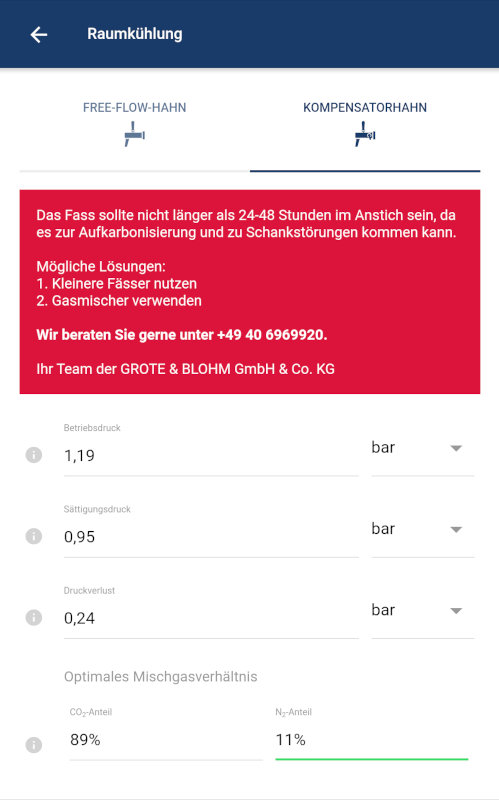
\includegraphics[width=4.8cm]{images/groteblohm.jpg}
%\caption{FOBB-APP}
%\label{fig:groteblohm}
%\end{figure}


\printbibliography[title=Quellen]

\end{document}